\documentclass{article}

\usepackage{GOST}
\usepackage[T1, T2A]{fontenc}
\usepackage[utf8]{inputenc}
\usepackage[russian]{babel}
\usepackage{cmap}
\usepackage{amssymb}
\usepackage{amsmath}
\usepackage{hyperref}

\usepackage{listings}
% Для листинга кода:
\lstset{ 
	language=C,                 % выбор языка для подсветки (здесь это С)
	basicstyle=\small\sffamily, % размер и начертание шрифта для подсветки кода
	numbers=left,               % где поставить нумерацию строк (слева\справа)
	numberstyle=\tiny,           % размер шрифта для номеров строк
	stepnumber=1,                   % размер шага между двумя номерами строк
	numbersep=5pt,                % как далеко отстоят номера строк от подсвечиваемого кода
	showspaces=false,            % показывать или нет пробелы специальными отступами
	showstringspaces=false,      % показывать или нет пробелы в строках
	showtabs=false,             % показывать или нет табуляцию в строках
	frame=single,              % рисовать рамку вокруг кода
	tabsize=2,                 % размер табуляции по умолчанию равен 2 пробелам
	captionpos=t,              % позиция заголовка вверху [t] или внизу [b] 
	breaklines=true,           % автоматически переносить строки (да\нет)
	breakatwhitespace=false, % переносить строки только если есть пробел
}


\graphicspath{{images/}}

\linespread{1.5}

\title{Отчет по анализу алгоритмов}
\date{2020}
\author{Pavel Khetagurov}

\begin{document}
	\begin{table}[ht]
	\centering
	\begin{tabular}{|c|p{400pt}|} 
	\hline
		\begin{tabular}[c]{@{}c@{}} 
\includegraphics[scale=0.15]{EmblemBMSTU} \\\end{tabular} &
		\footnotesize\begin{tabular}[c]{@{}c@{}}\textbf{Министерство~науки~и~высшего~образования~Российской~Федерации}\\\textbf{Федеральное~государственное~бюджетное~образовательное~учреждение}\\\textbf{~высшего~образования}\\\textbf{«Московский~государственный~технический~университет}\\\textbf{имени~Н.Э.~Баумана}\\\textbf{(национальный~исследовательский~университет)»}\\\textbf{(МГТУ~им.~Н.Э.~Баумана)}\\\end{tabular}  \\
	\hline
	\end{tabular}
\end{table}
\noindent\rule{\textwidth}{4pt}
\noindent\rule[14pt]{\textwidth}{1pt}
\hfill 
\noindent
\makebox{ФАКУЛЬТЕТ~}%
\makebox[\textwidth][l]{\underline{~~~~«Информатика и системы управления»~~~~~~~~~~~~~~~~~~~~~~~~~~~~~~~~~~~~~~~~~~~~}}%
\\
\noindent
\makebox{КАФЕДРА~}%
\makebox[\textwidth][l]{\underline{~~~~~~~«Программное обеспечение ЭВМ и информационные технологии»~~~~~~~~}}%
\\


\begin{center}
	\vspace{3cm}
	{\bf\huge Отчёт\par}
	{\bf\Large по лабораторной работе №7\par}
	\vspace{0.5cm}
\end{center}


\noindent
\makebox{\large{\bf Название:}~~~}
\makebox[\textwidth][l]{\large\underline{~Поиск в словаре~~~~~~~~~~~~~}}\\

\noindent
\makebox{\large{\bf Дисциплина:}~~~}
\makebox[\textwidth][l]{\large\underline{~Анализ алгоритмов~~~~~~~~~~~~~~~~~~~~~~~~~~~~~~~~~~~~~~~~~~~~~~~~~~~~}}\\

\vspace{1.5cm}
\noindent
\begin{tabular}{l c c c c c}
    Студент      & ~ИУ7-55Б~               & \hspace{3.5cm} & \hspace{3.5cm}                 & &  Хетагуров П.К \\\cline{2-2}\cline{4-4} \cline{6-6} 
    \hspace{3cm} & {\footnotesize(Группа)} &                & {\footnotesize(Подпись, дата)} & & {\footnotesize(И.О. Фамилия)}
\end{tabular}

\vspace{1cm}

\noindent
\begin{tabular}{l c c c c}
    Преподователь & \hspace{6cm}   & \hspace{3.5cm}                 & & Л.Л. Волкова \\\cline{3-3} \cline{5-5} 
    \hspace{3cm}  &                & {\footnotesize(Подпись, дата)} & & {\footnotesize(И.О. Фамилия)}
\end{tabular}

\begin{center}	
	\vfill
	\large \textit {Москва, 2020}
\end{center}

\thispagestyle {empty}
\pagebreak
	\newpage
	\tableofcontents
	\newpage
	\begin{center}
	    \section*{Введение}
	\end{center}
	\addcontentsline{toc}{section}{Введение}
		\indent \indent В данной лабораторной работе будут рассмотренны и проанализированы параллельные реализации алгоритма Винограда. Проведено сравнение рассмотренных параллельных алгоритмов с последовательной версией алгоритма Винограда.
	\newpage
	\section{Аналитическая часть}
	В данном разделе будут поставлены цели и задачи работы, будут рассмотренны основные теоритические сведения связанные с алгоритмами сортировки.
		\subsection{Цель и задачи работы}
			\textbf{Цель работы:}
			\newline
			Научиться работать с параллельными вычислениями.
			\newline 
			\indent \textbf{Задачи работы:}
			\begin{enumerate}
				\item разработать две параллельные версии алгоритма Винограда;
				\item реализовать разработанные алгоритмы и последовательный алгоритм Винограда;
				\item провести эксперименты по замеру времени работы разработанных алгоритмов;
				\item провести сравнения алгоритмов по затраченному времени.
			\end{enumerate}

		\subsection{Классическое умножение матриц}
		Операция умножения двух матриц выполнима тогда и только тогда, когда число
столбцов в первом сомножителе равно числу строк во втором.
\newline
\indent				Произведением матрицы A[m×n] на матрицу B[n×k] называется матрица C[m×k] такая,
			что элемент матрицы C, стоящий в i-ой строке и j-ом столбце, т. е. элемент $c_{i,j}$, равен сумме
			произведений элементов i-ой строки матрицы A на соответствующие элементы j-ого столбца
матрицы B. Т.е определяется формулой \hyperref[classicMultiply]{(\ref{classicMultiply})}:
			\begin{equation}\label{classicMultiply}
			c_{i,j} = \sum_{r=1}^{m}a_{ir}b_{rj} \qquad (i=1,2,...l; j = 1,2,...n)
			 \end{equation}
		\subsection{Последовательный алгоритм Винограда}
		Видно, что каждый элемент в результате умножения матриц представляет собой скалярное произведение соответствующих строки и столбца матриц. В алгоритме Винограда происходит некоторая предварительная обработка, позволяющая вычислить часть данных заранее. Заметим, что скалярное произведение двух векторов V и W, например, размерностью 4, можно переписать как \hyperref[vwOpen]{(\ref{vwOpen})}:
		\begin{equation}\label{vwOpen}
		V * W = (v_{1} + w_{2})(v_{2} + w_{1}) + (v_{3} + w_{4})(v_{4} + w_{3}) -  v_{1}v_{2} - v_{3}v_{4} - w_{1}w_{2} - w_{3}w_{4}
	\end{equation}
	\indent В случае матрицы со стороной нечетной длины, необходимо прибавить сделать коррекцию: $result[i, j] += first[i, m1 - 1] * second[m1 - 1, j]$
	\newline \indent Видно, что выражение в правой части допускает предварительную обработку, его части можно вычислить заранее и запомнить для каждой строки первой матрицы и для каждого столбца второй \cite{vinogradRef}.

	\subsection{Параллельные реализации алгоритма Винограда}
Алгоритм Винограда можно разделить на 4 части:
\begin{enumerate}
\item подготовка вектора mulH;
\item подготовка вектора mulV;
\item основной цикл;
\item цикл, вносящий поправки в вычисление.
\end{enumerate}
Следовательно, параллельные реализации могут быть следующими:
\begin{enumerate}
\item распараллеливание каждой из частей алгоритма, причем первые две могут выполняться одновременно;
\item распараллеливание только основного цикла, так как он занимает наибольшую часть времени выполнения.
\end{enumerate}
	\subsection{Вывод}
	В данной части были поставлены задачи и цель работы, рассмотрен классический  алгоритм умножения матриц, алгоритм Винограда и способы его распараллеливания.
		
	\newpage
	\section{Конструкторская часть}
		В данном разделе будут рассмотренны схемы алгоритмов, требования к функциональности ПО.
		\subsection{Требования к ПО} 
		ПО должно иметь два режима работы, выбираемых из меню
		\begin{enumerate}
			\item Режим демонстрации. В этом режиме должен осуществляться ввод матрицы и демонстрация работы на ней всех реализованных алгоритмов.
		 	\item Режим тестирования. В этом режиме должны проводится замеры времени выполнения реализованных алгоритмов в зависимости от количества потоков и размера матриц. Должен осуществляться вывод затраченного процессорного времени на случайным образом сгенерированных данных.
	 	\end{enumerate}
	 	
	 	\subsection{Схема алгоритма Винограда}
	 	
	На \hyperref[vinogradAlgo]{рисунке  \ref{vinogradAlgo}} изображена схема алгоритма Винограда.
	\begin{figure}[h!]
		\center{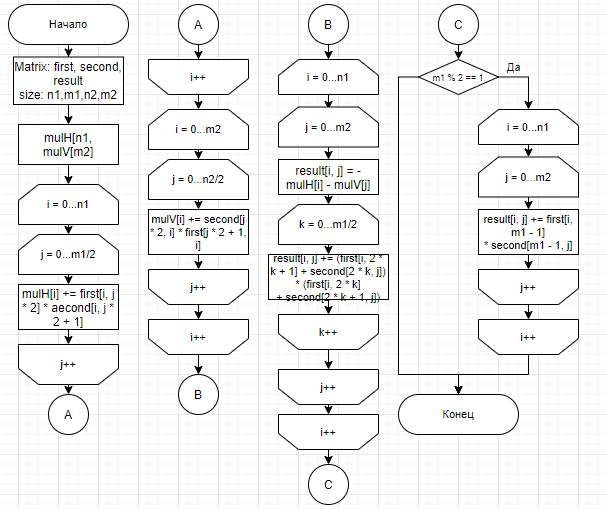
\includegraphics{vinogradAlgo.png}}
		\caption{Схема алгоритма Винограда}
		\label{vinogradAlgo}
	\end{figure}
	\newpage
		\subsection{Параллельные модификации}
		В первой параллельной реализации будут распараллелены все части алгоритма, а так же части A и B(расчет массивов) будут выполняться параллельно. Расспаралеливание частей A, B, C, D будет заключаться в делегировании процессу обработки части массива или матрицы, распределения зон ответственности. На \hyperref[firstParallel]{рисунке  \ref{firstParallel}} изображена схема данной параллельной реализации.
\begin{figure}[h!]
		\center{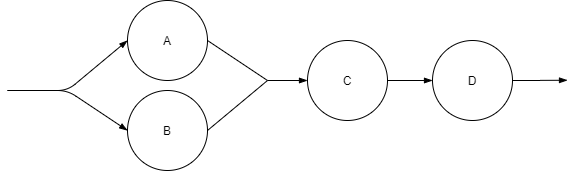
\includegraphics[scale=0.7]{firstParallel.png}}
		\caption{Первый вариант распараллеливания}
		\label{firstParallel}
	\end{figure}
\newline
		\indent Во второй параллельной реализации будет распараллелена только часть C(главный цикл). На \hyperref[secondParallel]{рисунке  \ref{secondParallel}} изображена схема второй параллельной реализации.
\begin{figure}[h!]
		\center{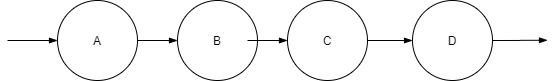
\includegraphics[scale=0.7]{secondParallel.png}}
		\caption{Второй вариант распараллеливания}
		\label{secondParallel}
	\end{figure}
	\subsection{Вывод}
	В данном разделе были рассмотрены схемы алгоритмов и обозначены требования к ПО.
	
	\newpage
	\section{Технологическая часть}
	Ниже будут представлены средства реализации и листинги реализованной программы.
	\subsection{Средcтва реализации}
	Выбранный язык программирования - C\#, так как требований по конкретнему языку не выдвигалось и он предоставляет удобные средства распараллеливания \cite{c-parallel}. Среда разработки - Visual Studio \cite{vs}.
\newline
	\indent Технические характеристики машины, на которой проводились тесты:
	\begin{itemize}
	\item Windows 10 x64;
	\item 8 ГБ оперативной памяти;
	\item CPU: AMD FX(tm)-6350 Six-Core Processor 3.90GHz;
	\item 6 логических ядер.
	\end{itemize}	
	\subsection{Реализации алгоритмов}
	Ниже представлены листинги реализаций алгоритмов.
	На листинге \hyperref[vinogradLst]{\ref{vinogradLst}} представлен алгоритм Винограда.
	\begin{lstlisting}[label=vinogradLst, caption=Алгоритм Винограда]
	public static Matrix Classic(Matrix first, Matrix second)
        {
            Matrix result = new Matrix(0, 0);
            if (first.M == second.N && first.N != 0 && second.M != 0)
            {
                int n1 = first.N;
                int m1 = first.M;
                int n2 = second.N;
                int m2 = second.M;

                result = new Matrix(n1, m2);
                int[] mulH = new int[n1];
                int[] mulV = new int[m2];

                for (int i = 0; i < n1; i++)
                {
                    for (int j = 0; j < m1 / 2; j++)
                    {
                        mulH[i] += first[i, j * 2] * first[i, j * 2 + 1];
                    }
                }

                for (int i = 0; i < m2; i++)
                {
                    for (int j = 0; j < n2 / 2; j++)
                    {
                        mulV[i] += second[j * 2, i] * second[j * 2 + 1, i];
                    }
                }

                for (int i = 0; i < n1; i++)
                {
                    for (int j = 0; j < m2; j++)
                    {
                        result[i, j] = -mulH[i] - mulV[j];
                        for (int k = 0; k < m1 / 2; k++)
                        {
                            result[i, j] += (first[i, 2 * k + 1] + second[2 * k, j]) * (first[i, 2 * k] + second[2 * k + 1, j]);
                        }
                    }
                }

                if (m1 % 2 == 1)
                {
                    for (int i = 0; i < n1; i++)
                    {
                        for (int j = 0; j < m2; j++)
                        {
                            result[i, j] += first[i, m1 - 1] * second[m1 - 1, j];
                        }
                    }
                }
            }

            return result;
        }
	\end{lstlisting}
		На листинге \hyperref[firstParallelLst]{\ref{firstParallelLst}} представлен первый вариант распараллеливания алгоритм Винограда.
	\begin{lstlisting}[label=firstParallelLst,caption=Первый вариант распараллеливания алгоритм Винограда]
public static Matrix ParallelFirst(Matrix first, Matrix second, int threadsCount)
        {
            Matrix result = new Matrix(0, 0);
            if (threadsCount <= 1)
            {
                result = Classic(first, second);
            }
            else if (first.M == second.N && first.N != 0 && second.M != 0)
            {
                int n1 = first.N;
                int m1 = first.M;
                int n2 = second.N;
                int m2 = second.M;

                result = new Matrix(n1, m2);
                int[] mulH = new int[n1];
                int[] mulV = new int[m2];

                Thread[] threads = new Thread[threadsCount];

                int threadsHalfing = threadsCount / 2;

                // mulH
                int threadWork = threadsHalfing;
                int step = n1 / threadWork;
                if (threadWork / n1 >= 1)
                {
                    step = 1;
                    threadWork = n1;
                    threadsHalfing = threadWork;
                }
                int start = 0;
                for (int i = 0; i < threadWork - 1; i++)
                {
                    threads[i] = new Thread(CountMulH);
                    threads[i].Start(new ParametersForMul(first, mulH, start, start + step, m1));
                    start += step;
                }
                threads[threadWork - 1] = new Thread(CountMulH);
                threads[threadWork - 1].Start(new ParametersForMul(first, mulH, start, n1, m1));

                // MulV
                threadWork = (threadsCount - threadsHalfing);
                step = m2 / threadWork;
                if (threadWork / m2 >= 1)
                {
                    step = 1;
                    threadWork = m2;
                }
                start = 0;
                for (int i = threadsHalfing; i < threadsHalfing + threadWork - 1; i++)
                {
                    threads[i] = new Thread(CountMulV);
                    threads[i].Start(new ParametersForMul(second, mulV, start, start + step, n2));
                    start += step;
                }
                threads[threadsHalfing + threadWork - 1] = new Thread(CountMulV);
                threads[threadsHalfing + threadWork - 1].Start(new ParametersForMul(second, mulV, start, m2, n2));

                //sync
                for (int i = 0; i < threadWork + threadsHalfing; i++)
                {
                    threads[i].Join();
                }

                //Main
                step = n1 / threadsCount;
                threadWork = threadsCount;
                if (threadsCount / n1 >= 1)
                {
                    step = 1;
                    threadWork = n1;
                }
                start = 0;
                for (int i = 0; i < threadWork - 1; i++)
                {
                    threads[i] = new Thread(CountMain);
                    threads[i].Start(new ParametersForMain(result, first, second, mulV, mulH, start, start + step, m2, m1));
                    start += step;
                }
                threads[threadWork - 1] = new Thread(CountMain);
                threads[threadWork - 1].Start(new ParametersForMain(result, first, second, mulV, mulH, start, n1, m2, m1));

                // sync
                for (int i = 0; i < threadWork; i++)
                {
                    threads[i].Join();
                }

                // end
                if (m1 % 2 == 1)
                {
                    start = 0;
                    for (int i = 0; i < threadWork - 1; i++)
                    {
                        threads[i] = new Thread(CountTail);
                        threads[i].Start(new ParametersForMain(result, first, second, mulV, mulH, start, start + step, m2, m1));
                        start += step;
                    }
                    threads[threadWork - 1] = new Thread(CountTail);
                    threads[threadWork - 1].Start(new ParametersForMain(result, first, second, mulV, mulH, start, n1, m2, m1));

                    // sync
                    for (int i = 0; i < threadWork; i++)
                    {
                        threads[i].Join();
                    }
                }
            }

            return result;
        }
	\end{lstlisting}
		На листинге \hyperref[secondParallelLst]{\ref{secondParallelLst}} представлен второй вариант распараллеливания алгоритм Винограда.
	\begin{lstlisting}[label=secondParallelLst,caption=Второй вариант распараллеливания алгоритм Винограда]
public static Matrix ParallelSecond(Matrix first, Matrix second, int threadsCount)
        {
            Matrix result = new Matrix(0, 0);
            if (threadsCount <= 1)
            {
                result = Classic(first, second);
            }
            else if (first.M == second.N && first.N != 0 && second.M != 0)
            {
                int n1 = first.N;
                int m1 = first.M;
                int n2 = second.N;
                int m2 = second.M;

                result = new Matrix(n1, m2);
                int[] mulH = new int[n1];
                int[] mulV = new int[m2];

                for (int i = 0; i < n1; i++)
                {
                    for (int j = 0; j < m1 / 2; j++)
                    {
                        mulH[i] += first[i, j * 2] * first[i, j * 2 + 1];
                    }
                }

                for (int i = 0; i < m2; i++)
                {
                    for (int j = 0; j < n2 / 2; j++)
                    {
                        mulV[i] += second[j * 2, i] * second[j * 2 + 1, i];
                    }
                }

                //Main
                Thread[] threads = new Thread[threadsCount];
                int step = n1 / threadsCount;
                int threadWork = threadsCount;
                if (threadsCount / n1 >= 1)
                {
                    step = 1;
                    threadWork = n1;
                }
                int start = 0;
                for (int i = 0; i < threadWork - 1; i++)
                {
                    threads[i] = new Thread(CountMain);
                    threads[i].Start(new ParametersForMain(result, first, second, mulV, mulH, start, start + step, m2, m1));
                    start += step;
                }
                threads[threadWork - 1] = new Thread(CountMain);
                threads[threadWork - 1].Start(new ParametersForMain(result, first, second, mulV, mulH, start, n1, m2, m1));

                // sync
                for (int i = 0; i < threadWork; i++)
                {
                    threads[i].Join();
                }

                // end
                if (m1 % 2 == 1)
                {
                    for (int i = 0; i < n1; i++)
                    {
                        for (int j = 0; j < m2; j++)
                        {
                            result[i, j] += first[i, m1 - 1] * second[m1 - 1, j];
                        }
                    }
                }
            }

            return result;
        }
\end{lstlisting}
На листинге \hyperref[helpLst]{\ref{helpLst}} представлены вспомогательные функции.
	\begin{lstlisting}[label=helpLst,caption=Вспомогательные функции]
private static void CountMulH(object paramsObj)
        {
            ParametersForMul paramses = (ParametersForMul)paramsObj;
            int start = paramses.start,
                end = paramses.end,
                secondBorder = paramses.secondBorder;
            Matrix matrix = paramses.matrix;
            int[] mul = paramses.array;

            for (int i = start; i < end; i++)
            {
                for (int j = 0; j < secondBorder / 2; j++)
                {
                    mul[i] += matrix[i, j * 2] * matrix[i, j * 2 + 1];
                }
            }
        }

        private static void CountMulV(object paramsObj)
        {
            ParametersForMul paramses = (ParametersForMul)paramsObj;
            int start = paramses.start,
                end = paramses.end,
                secondBorder = paramses.secondBorder;
            Matrix matrix = paramses.matrix;
            int[] mul = paramses.array;

            for (int i = start; i < end; i++)
            {
                for (int j = 0; j < secondBorder / 2; j++)
                {
                    mul[i] += matrix[j * 2, i] * matrix[j * 2 + 1, i];
                }
            }
        }

        private static void CountMain(object paramsObj)
        {
            ParametersForMain paramses = (ParametersForMain)paramsObj;
            Matrix result = paramses.result,
                first = paramses.first,
                second = paramses.second;
            int[] mulH = paramses.mulH,
                mulV = paramses.mulV;
            int start = paramses.start,
                end = paramses.end,
                m2 = paramses.m2,
                m1 = paramses.m1;

            for (int i = start; i < end; i++)
            {
                for (int j = 0; j < m2; j++)
                {
                    result[i, j] = -mulH[i] - mulV[j];
                    for (int k = 0; k < m1 / 2; k++)
                    {
                        result[i, j] += (first[i, 2 * k + 1] + second[2 * k, j]) * (first[i, 2 * k] + second[2 * k + 1, j]);
                    }
                }
            }
        }

        private static void CountTail(object paramsObj)
        {
            ParametersForMain paramses = (ParametersForMain)paramsObj;
            Matrix result = paramses.result,
                first = paramses.first,
                second = paramses.second;
            int start = paramses.start,
                end = paramses.end,
                m2 = paramses.m2,
                m1 = paramses.m1;

            for (int i = start; i < end; i++)
            {
                for (int j = 0; j < m2; j++)
                {
                    result[i, j] += first[i, m1 - 1] * second[m1 - 1, j];
                }
            }
        }
	\end{lstlisting}

	\subsection{Вывод}
	В данном разделе были описаны программные и аппаратные средства реализации, были представлены листинги реализаций алгоритмов.

	\newpage
	\section{Экспериментальная часть}
	В данной главе будет представлен пример работы программы, результат экспериментов по замеру времени и произведен сравнительный анализ алгоритмов по затрачиваемому времени.
	\subsection{Пример работы программы}
	Пример работы программы представлен на рисунке \hyperref[programmWork]{\ref{programmWork}}
	 	\begin{figure}[h!]
		 	\center{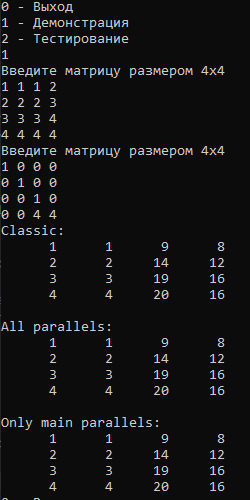
\includegraphics[scale=0.9]{programmWork.png}}
		 	\caption{Пример работы программы}
		 	\label{programmWork}
	 	\end{figure}
	
	\subsection{Сравнительный анализ алгоритмов по времени}
	Эксперимент проводится на матрице размером 500x500. Количество потоков варьируется от 1 до 24 с шагом 2. Количество потоков не влияет на последовательную реализацию алгоритма, поэтому её график не отражает зависимость между скоростью выполнения и количеством потоков, а приведен для сравнения.  Результаты представлены на рисунке \hyperref[test_mylt]{\ref{test_mylt}}.
	\begin{figure}[h!]
		 	\center{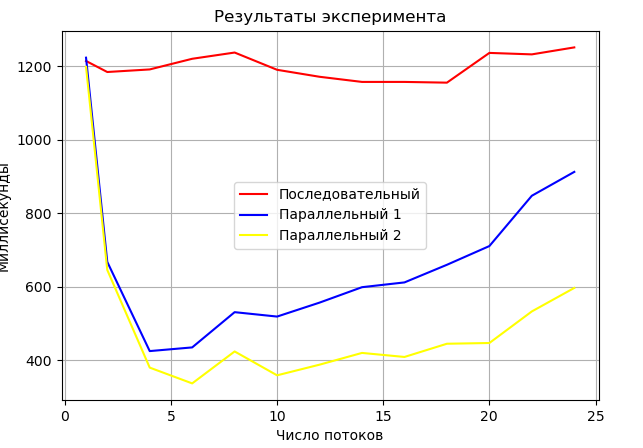
\includegraphics{test_mylt.png}}
		 	\caption{Результаты на разном количестве потоков}
		 	\label{test_mylt}
	 	\end{figure}
	\newpage
	На рисунке \hyperref[test_fix]{\ref{test_fix}} представлено сравнение алгоритмов на 6 потоках(кроме последовательной реализации) на матрицах со сторонами от 10 до 1000 с шагом 99.
	\begin{figure}[h!]
		 	\center{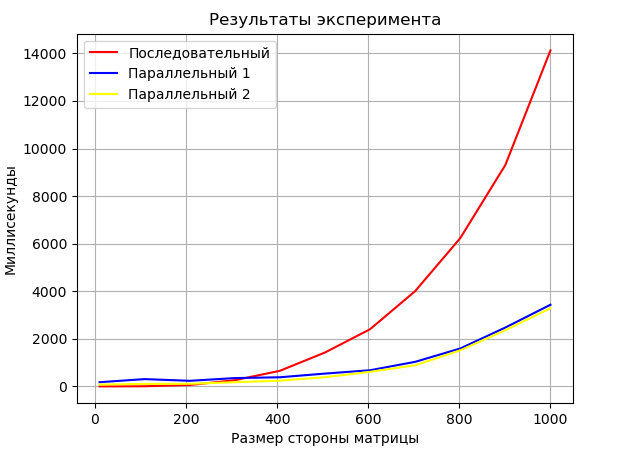
\includegraphics{test_fix.png}}
		 	\caption{Результаты на разных размерах матриц}
		 	\label{test_fix}
	 	\end{figure}
	\newpage
	\subsection{Вывод}
	Как видно из графиков, самой долгой реализацией является последовательная версия алгоритма. 
	Самой быстрой является первая версия параллельного алгоритма. Вторая версия быстрее 
	последовательной, но уступает в скорости работы второй.
	\newline
	\indent Так же видно, что при увеличении количества потоков от 1 до 6 параллельные версии алгоритмов работают все быстрее, но на количестве потоков больше 6 алгоритмы начинают немного замедляться. Это объясняется тем, что 6 - количество логических ядер машины, на которой проводились тесты, и, при количестве потоков больше 6, реализуется псевдопараллельность, которая занимает больше времени из-за смены контекстов.

	\newpage
	\begin{center}
		\section*{Заключение}
	\end{center}
	\addcontentsline{toc}{section}{Заключение}
	\indent \indent В данной лабораторной работе были разработаны параллельные алгоритмы Винограда. Они были реализованы, а также были проведены эксперименты по замеру времени работы реализованных алгоритмов и проведены сравнения алгоритмов по результатам эксперимента. Цель работы достигнута, все задачи выполнены.
	\newpage
	\addcontentsline{toc}{section}{Список литературы}
	
	\begin{center}
	\begin{thebibliography}{3}
	\bibitem{vinogradRef}
	Умножение матриц [Электронный ресурс]. Режим доступа: (дата обращения - 02.10.2020) Свободный. URL: http://www.algolib.narod.ru/Math/Matrix.html
	\bibitem{c-parallel}
	API.NET. Пространство имен System.Threading [Электронный ресурс]. Режим доступа: (дата обращения - 28.10.2020) Свободный. URL: https://docs.microsoft.com/ru-ru/dotnet/api/system.threading?view=netcore-3.1
	\bibitem{vs}
	Visual Studio [Электронный ресурс]. Режим доступа: (дата обращения - 28.10.2020) Свободный. URL: https://visualstudio.microsoft.com/ru/

	\end{thebibliography}
	\end{center}
\end{document}